\subsection{iSAM2}
\subsubsection{Introduction and Motivation}
\gls{iSAM}2 was developed to overcome the practical limitations of \gls{iSAM}. The core optimization method in \gls{iSAM} (nonlinear least squares solved through incremental QR factorization) is sound and provides accurate solutions. The bottlenecks arise not from the underlying algorithms, but from the static data structure used to maintain the problem. In \gls{iSAM} the system is stored as a single global square root information matrix $R$. While this representation is compact and efficient for batch updates, it leads to several issues during incremental operation.
\\ \\
First, the $R$ matrix is ``global''. Adding new factors or loop closures often changes many rows and columns, which requires expensive refactorization. This causes latency spikes, especially when loop closures occur and large parts of the trajectory suddenly become coupled. Second, relinearization in \gls{iSAM} is also global. To maintain accuracy, the system periodically refreshes Jacobians for all factors, which forces full reconstruction of the $R$ matrix. Third, variable reordering to reduce fill in and keep $R$ sparse is again an all or nothing operation, with cost proportional to the entire problem size. Together, these properties mean that \gls{iSAM}, while efficient between updates, still suffers from periodic heavy computation that disrupts real time performance.
\\ \\
\gls{iSAM}2 addresses these limitations by introducing a new data structure, the ``Bayes tree''. Instead of representing the system as a static $R$ matrix, \gls{iSAM}2 leverages the factor graph formulation of \gls{SLAM}, applies variable elimination, and interprets the resulting structure as a chordal Bayes net. This Bayes net can then be compactly represented as a Bayes tree, which retains all probabilistic information while enabling local updates. With the Bayes tree, adding new measurements or relinearizing states only modifies the affected cliques in the tree, leaving the rest untouched. This local property eliminates the global refactorization bottlenecks of \gls{iSAM}, smooths out computation over time, and makes the algorithm scalable to large and long term mapping problems. \cite{iSAM2_paper,Bayes_tree_for_SLAM_paper}



\subsubsection{Factor Graphs}
A factor graph is a bipartite graph that connects variable nodes (poses and landmarks) to factor nodes (priors, motion, and measurements). It encodes the same estimation problem as in \gls{iSAM}, but makes sparsity and locality explicit because each factor touches only a few variables.
\\ \\
If we let the variables be robot poses $x_1,\dots,x_M$ and landmarks $l_1,\dots,l_N$, and let $\Theta=\{x_1,\dots,x_M,l_1,\dots,l_N\}$. According to the \gls{iSAM}2 papers \cite{iSAM2_paper,Bayes_tree_for_SLAM_paper} the posterior factorizes as
\[
    f(\Theta) = \prod_{i} f_i(\Theta_i),
\]
Here, each factor $f_i$ depends only on its adjacent variables $\Theta_i$. The way we model each factor depends on the situation, however since we are dealing with real world where our odometry and measurement variables are uncertain, we should use a probabilistic model to represent factors. One of the easiest probabilistic models is Gaussian, which is easy to model and will work well later when working in Mahalanobis form to optimize the problem and solve it in simple manner (See Figure \ref{fig:mahalanobis-distance} for Mahalanobis form). Factor functions can therefore be modeled as follows:
\[
    \text{Prior:}\quad f_p(x_0)\ \propto\ \exp\!\Big(-\tfrac{1}{2}\|\mu_0 - x_0\|_{P_0}^2\Big),
\]
\[
    \text{Odometry:}\quad f_i(x_{i-1},x_i)\ \propto\ \exp\!\Big(-\tfrac{1}{2}\|f_i(x_{i-1},u_i) - x_i\|_{Q_i}^2\Big),
\]
\[
    \text{Measurement:}\quad f_k(x_{i_k},l_{j_k})\ \propto\ \exp\!\Big(-\tfrac{1}{2}\|h_k(x_{i_k},l_{j_k}) - z_k\|_{R_k}^2\Big).
\]
This is in a way very similar to how \gls{iSAM} models the system, however here in \gls{iSAM}2, the system is represented as factor graphs. This graph view exposes conditional independence directly in the topology. Each factor only connects nearby variables in time or space, which later yields a sparse linear system.
\\ \\
\begin{figure}[H]
    \centering
    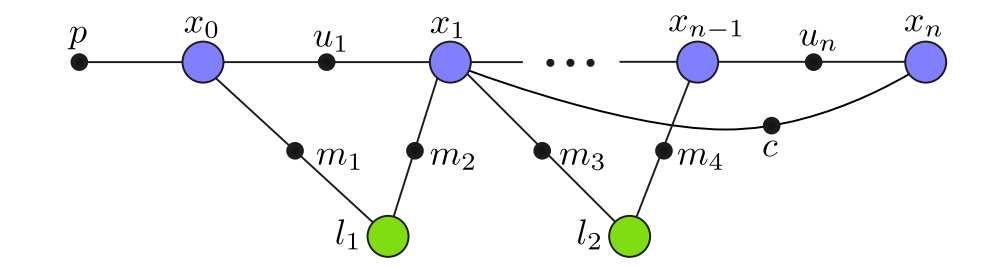
\includegraphics[width=0.98\linewidth]{Pictures/Optimizers/iSAM2/Factor_graph.png}
    \caption{Picture from \gls{iSAM}2 paper \cite{iSAM2_paper} describes factor graph formulation of the \gls{SLAM} problem. Variable nodes (large circles) are poses $x_0,\dots,x_n$ and landmarks $l_1,l_2$. Factor nodes (small solid circles) represent a prior $p$, odometry $u_i$, landmark measurements $m_i$, and a loop closure constraint $c$. We can represent any cost function, including factors that connect more than two variables.}
    \label{fig:optimizer-iSAM2-factor-graph}
\end{figure}
\noindent
This example shows how local connectivity induces sparsity. This will be useful when solving the optimization problem later down bellow. Each factor touches only its adjacent variables, so after linearization (to compute a local optimum) the Jacobian rows have nonzeros only in those columns. The resulting matrix is sparse, which helps the optimizer.



\subsubsection{From Factor Graphs to the SLAM Optimization Problem}
We represent \gls{SLAM} with a factor graph $G=(\mathcal{F},\Theta,\mathcal{E})$. There are two node types, factor nodes $f_i\in\mathcal{F}$ that encode pieces of information (prior, odometry, measurements, loop closures), and variable nodes $\theta_j\in\Theta$ that hold unknowns (poses, landmarks, calibration). An edge $e_{ij}\in\mathcal{E}$ is drawn only when factor $f_i$ depends on variable $\theta_j$. This wiring is important, missing edges mean independence, and the pattern of edges controls which variables interact in the estimation problem.
\\ \\
The graph specifies how a global objective splits into simple parts:
\[
    f(\Theta)\;=\;\prod_i f_i(\Theta_i),
\]
Here $\Theta_i$ collects only the variables that touch factor $f_i$. In the \gls{SLAM} setting, a prior $p$ anchors the first pose, odometry factors $u$ relate consecutive poses, landmark factors $m$ couple a pose with a landmark, and loop closure factors $c$ link poses that see the same place again (see Picture \ref{fig:optimizer-iSAM2-factor-graph}). The same framework can also handle factors that involve three or more variables, for example a factor that ties a pose to a landmark and a camera intrinsics block (calibration), or ``separator'' variables shared in cooperative mapping. The key point is that the graph can host any cost term as long as we state which variables it touches.
\\ \\
Under Gaussian measurement models as we defined in the previous subsection, each factor has the form:
\[
    f_i(\Theta_i)\ \propto\ \exp\!\Big(-\tfrac12\,\|\,h_i(\Theta_i)-z_i\,\|^2_{\Sigma_i}\Big),
\]
This Gaussian form will simplify calculations as Gaussian is nice to work with. Here $h_i(\cdot)$ predicts what the sensor should see from the current variables $\Theta_i$, $z_i$ is the actual measurement, and $\Sigma_i$ is the measurement covariance. The notation $\|e\|^2_{\Sigma}\triangleq e^\top \Sigma^{-1} e$ is the squared Mahalanobis distance, which measures error in ``units of its noise'' (directions with low variance are penalized more). (See Picture \ref{fig:mahalanobis-distance})
\\ \\
To combine all information, we multiply the factor likelihoods. Products are awkward to optimize, so we take a negative logarithm to turn the product into a sum. Terms that do not depend on $\Theta$ drop out, and each Gaussian factor becomes a squared Mahalanobis residual weighted by its covariance. The result is one scalar objective that collects the prior, all odometry factors, all landmark measurements, and any loop closures. Small covariances make a factor count more, large covariances count less. In short, multiply the factors and take the negative log to get a single sum of squared errors. We write it compactly as:
\[
    \Theta^\star \;=\;\arg\min_{\Theta}\ \frac12\sum_i \|\,h_i(\Theta_i)-z_i\,\|^2_{\Sigma_i}
\]
All variables (poses, landmarks, and any auxiliary parameters) live inside the same cost, and only variables that share a factor appear together in a residual, which later yields a sparse linear system when we linearize.
\\ \\
This is our \gls{MAP} function in nonlinear form.
\\ \\
We do not solve this nonlinear cost in one shot because $h_i(\cdot)$ measurement transform is nonlinear (because of angles, ranges, bearing-only sensors, etc...). Instead we solve it in similar fashion we solved \gls{iSAM} system model, we linearize and solve iteratively. Choose a current estimate $\Theta^0$ and look for a small update $\Delta\theta$ that improves the fit. For each factor we take a 1st-order Taylor expansion around $\Theta^0$, which turns that factor into a simple linear residual in the increment $\Delta\theta$ that touches only its adjacent variables. After whitening by $\Sigma_i^{-1/2}$, we stack all linearized factors into one sparse least-squares problem:
\begin{equation}
    \begin{aligned}
        \Delta\Theta^\star = \arg\min_{\Delta\Theta} \left( -log\left(f(\Delta\Theta)\right) \right) = \Delta\theta^\star = \arg\min_{\Delta\theta}\ \|A\,\Delta\theta - b\|^2
    \end{aligned}
    \label{eq:optimizer-iSAM2-least-square}
\end{equation}
Here $A\in\mathbb{R}^{m\times n}$ is the measurement Jacobian (one row block per factor), $b$ stacks the whitened prediction errors, and $\Delta\theta$ is the $n$-dimensional increment. The sparsity pattern of $A$ is dictated by the factor graph, a row has nonzeros only in the columns of the variables that appear in that factor.
\\ \\
What we can do here is solve this linear least squares problem in a numerically stable way. One route is the normal equations $A^\top A\,\Delta\theta = A^\top b$ and a Cholesky factorization $A^\top A = R^\top R$ followed by forward and back substitution to recover $\Delta\theta$. Another route is QR factorization on $A$, which yields an upper triangular system $R\,\Delta\theta = d$ that we solve by back substitution. Both routes are standard, in practice we prefer square-root methods (QR/Cholesky) for stability.
\\ \\
After solving for $\Delta\theta$, we update the state $\theta \leftarrow \theta + \Delta\theta$ and repeat, linearize, solve, update. This is Gauss-Newton. If the problem is difficult (poor linearization, strong nonlinearity), we add Levenberg-Marquardt damping and instead solve $(A^\top A + \lambda I)\Delta\theta = A^\top b$, which blends Gauss-Newton with a trust-region step to keep updates safe. We stop when $\Delta\theta$ is small or the cost no longer decreases.
\\ \\
This is the same least squares core as in \gls{iSAM}. The difference is the data structure. \gls{iSAM} works with the Jacobian $A$ and its triangular factor $R$. \gls{iSAM}2 keeps the factor graph as the main object, which carries the same information as $A$ but in a graph form. We eliminate variables to get a Bayes net and store it as a Bayes tree. This lets us update only the cliques touched by new factors instead of refactoring everything. In the next subsection we will see how it is done.



\subsubsection{From Factor Graphs to Bayes Networks}
\begin{figure}[H]
    \centering
    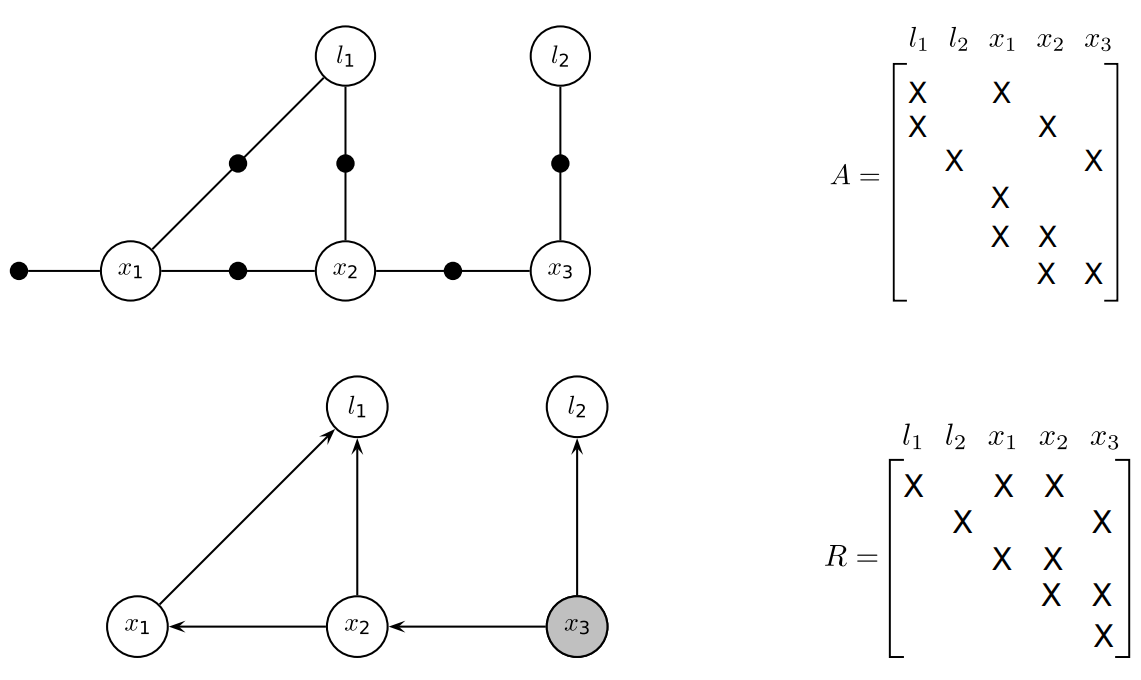
\includegraphics[width=0.98\linewidth]{Pictures/Optimizers/iSAM2/Factor_graph_to_Bayes_network.png}
    \caption{Picture from \gls{iSAM}2 paper \cite{iSAM2_paper}. (Top) factor graph and associated Jacobian $A$ for a small \gls{SLAM} example with poses $x_1,x_2,x_3$, landmarks $l_1,l_2$, and a prior on $x_1$ (Bottom) the chordal Bayes net and the square root factor $R$ obtained by eliminating in the order $l_1,l_2,x_1,x_2,x_3$. The last eliminated variable (the root) is shaded. \cite{iSAM2_paper}}
    \label{fig:optimizer-iSAM2-factor-graph-to-bayes-netwrok}
\end{figure}
\noindent
Starting from the least squares form in \eqref{eq:optimizer-iSAM2-least-square} we can factor the (whitened) measurement matrix $A$ exactly as in \gls{iSAM}. We pick an elimination order (for the example in Picture \ref{fig:optimizer-iSAM2-factor-graph-to-bayes-netwrok} it is $l_1,l_2,x_1,x_2,x_3$) and run sparse QR with Givens rotations \eqref{eq:optimizer-iSAM-givens-rotation}. This produces an orthogonal $Q$ and an upper triangular $R$. Because $R$ is triangular, solving by back substitution proceeds variable by variable in the chosen order. That solve can be read as a chain of simple Gaussian conditionals, one per variable, where the off diagonal entries to the right of each pivot indicate which previously eliminated variables that conditional depends on. If we draw arrows from those ``parent'' variables to the current one, the same structure becomes a directed graphical model. In short, for a chosen ordering, sparse QR on the factor graph yields an $R$ that encodes a Bayes network, this is what the bottom panel of Picture \ref{fig:optimizer-iSAM2-factor-graph-to-bayes-netwrok} shows.
\\ \\
Rather than running sparse QR on the whitened Jacobian, we can reach the same end result by eliminating variables directly on the factor graph by bipartite elimination game methods instead \cite{QR_factorization}. Starting from \eqref{eq:optimizer-iSAM2-least-square}, choose an order, then for each variable collect its adjacent factors, combine them, marginalize that variable out, and attach the resulting factor to the remaining neighbors. Repeat until all variables are removed. For any fixed order this purely graphical elimination produces exactly the same dependency pattern and the same square root information factor we would get from numeric QR factorization. This method directly forms a Bayes network with properties of chordal, and in the matrix view we obtain an upper triangular $R$ with $R^\top R = A^\top A$ (see Picture \ref{fig:optimizer-iSAM2-factor-graph-to-bayes-netwrok}). The advantage is that we never have to assemble $A$ or apply Givens rotations \eqref{eq:optimizer-iSAM-givens-rotation} and do QR factorization. We stay on the graph, let the ordering control fill, and arrive at the chordal structure we want. In practice this is the same QR algebra, just done in a graph aware way that avoids unnecessary intermediate fill and work according to Good Column Orderings for Sparse QR Factorization paper \cite{QR_factorization}.
\\ \\
This observation is the bridge to \gls{iSAM}2. A chordal Bayes network groups naturally into cliques, so we can represent it as a Bayes tree. In the next subsections we use this tree, instead of one global $R$, to support local updates and avoid global refactorizations.



\subsubsection{R as a Bayes tree data structure}
A key outcome of variable elimination on the \gls{SLAM} factor graph is a chordal Bayes network. Chordal means that in the moralized (undirected) view every long cycle has a shortcut edge, which keeps parents of a variable grouped in small cliques and prevents excessive fill in during elimination. This property is what makes the square root factor $R$ sparse and tractable, and it also sets up a clean bridge to a tree representation of the same information. \cite{iSAM2_paper,Bayes_tree_for_SLAM_paper}
\\ \\
\begin{figure}[H]
    \centering
    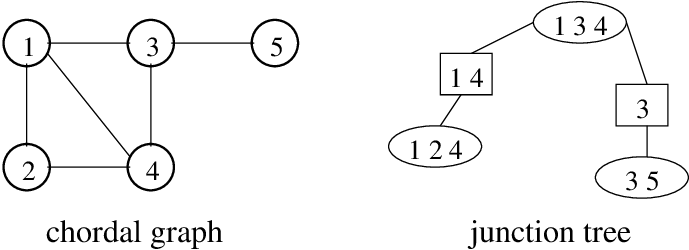
\includegraphics[width=0.98\linewidth]{Pictures/Optimizers/iSAM2/chodar_graph_to_junction_tree_example.png}
    \caption{Picture from Robert Castelo paper \cite{chordal_graph_to_junction_tree_paper} shows an example of a simple Chordal graph (Left side) and corresponding small cliques/junction tree (Right side). Eliminating in a good order produces a chordal Bayes net whose moralized graph can be grouped into cliques/junction trees. This is the structure that keeps $R$ matrix sparse.}
    \label{fig:optimizer-iSAM2-chordal}
\end{figure}
\noindent
When we linearize and eliminate in some order, the resulting triangular system $R$ still satisfies $R^\top R = A^\top A$, but each row block of $R$ matrix now carries a specific meaning. Each row block of $R$ belongs to the variable we just eliminated. That row says, in Gaussian form, how this variable depends on a few variables that were eliminated earlier. Think of those earlier variables as its parents. When we solve $R\Delta\theta=d$ by back substitution we start at the last row and move upward. That is the same as computing each variable from its parents in turn. So $R$ is not just numbers in a triangle. It is the same set of conditional relationships as the Bayes network, written in matrix form.
\\ \\
Because the Bayes net is chordal, its conditionals naturally group into cliques. If we collect consecutive row blocks of $R$ that share the same separator, each group is one clique. Connect two cliques when they share that separator, and we obtain a Bayes tree. Every clique node stores ``frontal $child|parent$ separator'' conditionals, and every edge carries only the shared separator variables. The tree therefore encodes the same numeric information as $R$, but organized by locality rather than by a single global ordering.
\\ \\
\begin{figure}[H]
    \centering
    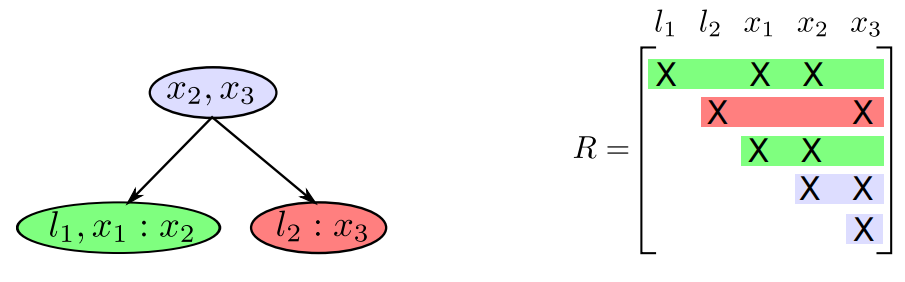
\includegraphics[width=0.98\linewidth]{Pictures/Optimizers/iSAM2/R_matrix_as_bayes_tree1.png}
    \caption{Picture from Bayes tree paper \cite{Bayes_tree_for_SLAM_paper} shows Bayes tree (left) and its matching rows in the square root factor $R$ (right). Colors indicate which contiguous row blocks of $R$ belong to each clique.}
    \label{fig:optimizer-iSAM2-R-to-tree-1}
\end{figure}
\begin{figure}[H]
    \centering
    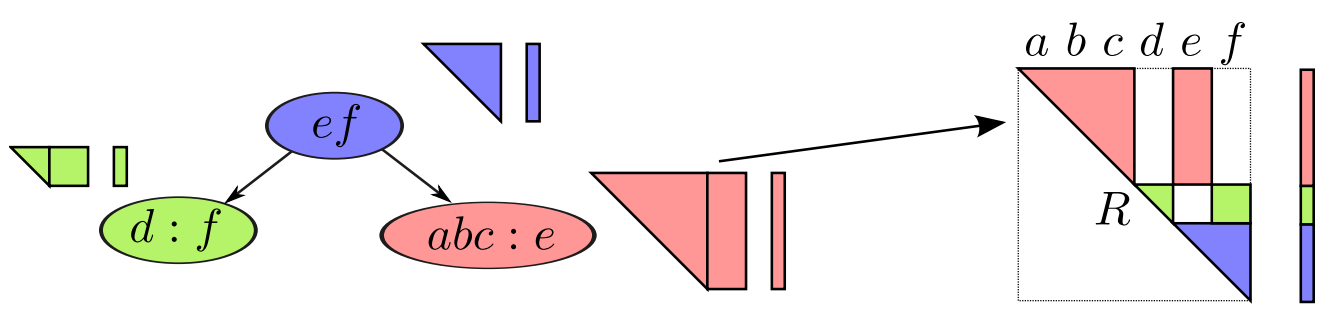
\includegraphics[width=0.98\linewidth]{Pictures/Optimizers/iSAM2/R_matrix_as_bayes_tree2.png}
    \caption{Picture from \gls{iSAM}2 paper \cite{iSAM2_paper} shows each clique contains the conditional of its frontal variables given the separator. The same entries appear in the corresponding rows/columns of $R$. Back substitution on $R$ mirrors evaluating the tree from leaves to root, while marginal queries follow the few cliques that touch the queried variables.}
    \label{fig:optimizer-iSAM2-R-to-tree-2}
\end{figure}
\noindent
The takeaway is simple. Eliminating a factor graph gives a chordal Bayes net. Grouping its conditionals yields a Bayes tree. The square root factor $R$ contains the very same conditionals in matrix form. Hence we can think of $R$ as a Bayes tree data structure written as a matrix. \gls{iSAM}2 stores and updates this Bayes tree directly instead of one global $R$, which preserves the numerical benefits of the square root form while enabling strictly local updates. This means when new measurements arrive or when some variables must be re-linearized, only the cliques on a small subtree are touched and the rest of the structure stays unchanged, making computational complexity manageable and the data set grows.



\subsubsection{Incremental Updates directly on Bayes tree}
In \gls{iSAM}2 we never rebuild the whole system when new data arrives. A new odometry or landmark factor only touches a few variables in the factor graph, so only the matching subtree in the Bayes tree is modified. All other branches stay exactly the same. This is the key difference from \gls{iSAM}, where adding a factor could force a global re-factorization of the single $R$ matrix.
\\ \\
Two simple rules explain why updates stay local. First is that information flows upward in the tree during elimination, so changes propagate only from the touched variables toward the root. Second, a factor becomes active when the first variable in its local elimination order is eliminated, so only the paths from those variables up to the root can be affected, while unrelated subtrees remain untouched.
\\ \\
\begin{figure}[H]
    \centering
    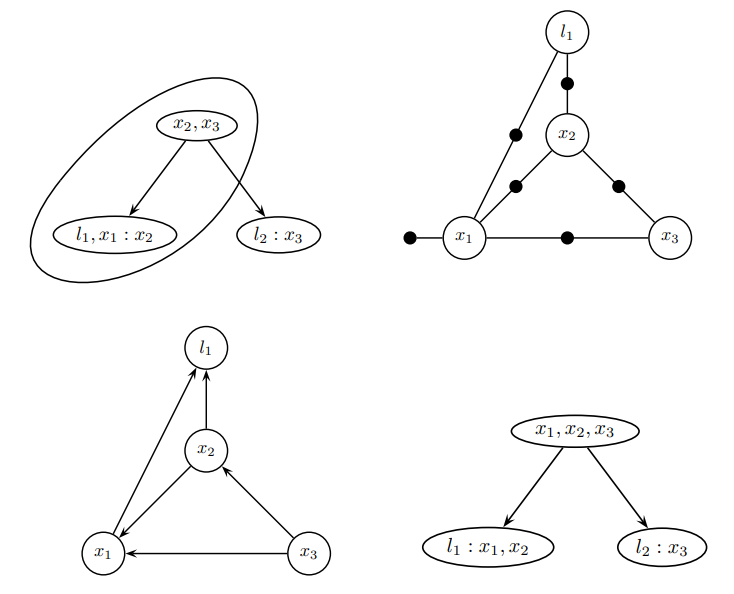
\includegraphics[width=0.98\linewidth]{Pictures/Optimizers/iSAM2/updating_Bayes_tree.png}
    \caption{Picture taken from Bayes tree paper \cite{Bayes_tree_for_SLAM_paper} shows how to update a Bayes tree with a new factor. \\ \noindent 
    (Top left) Affected cliques when adding a factor between $x_1$ and $x_3$, the right branch is unaffected. \\ \noindent
    (Top right) Local factor graph rebuilt from those cliques plus the new factor. \\ \noindent
    (Bottom left) Local chordal Bayes net after elimination. \\ \noindent
    (Bottom right) New Bayes subtree with the untouched ``orphan'' subtree reattached.}
    \label{fig:optimizer-iSAM2-R-update-tree}
\end{figure}
\noindent
One update works as follows. first, locate the cliques that contain the variables touched by the new factor and follow their ancestors up toward the root, this marks the only region that needs work, while the rest of the tree becomes ``orphans'' that stay valid and untouched. Next, convert the conditionals stored in those marked cliques back into a small local factor graph and insert the new factor. Then re-eliminate just this local graph (using the same graph aware elimination as discussed previously) to produce a new chordal Bayes net and its updated Bayes subtree. Finally, reattach the orphan subtrees at the proper separators. Only this small subtree changes, everything else is reused. (See Picture \ref{fig:optimizer-iSAM2-R-update-tree})
\\ \\
The result is incremental and predictable computation. \gls{iSAM}2 edits only the cliques touched by the new information, runs a small local elimination, and solves by back substitution along that subtree. There are no global re-factorization spikes, and accuracy is maintained because we can also re-linearize only the variables inside the same affected region when needed.



\subsubsection{Loop Closure and Incremental Reordering}
\begin{figure}[H]
    \centering
    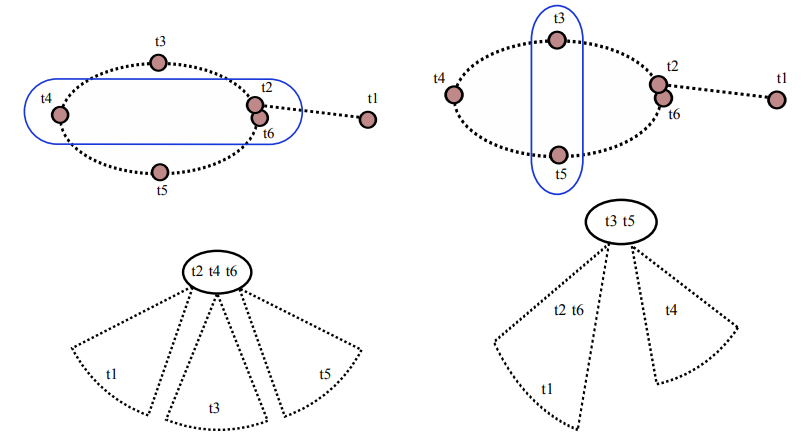
\includegraphics[width=0.98\linewidth]{Pictures/Optimizers/iSAM2/incremental_reordering.png}
    \caption{Picture taken from Bayes tree paper \cite{Bayes_tree_for_SLAM_paper} shows loop closure with incremental reordering. Two batch optimal orderings (top) yield different Bayes trees (bottom). For online operation we prefer the ordering that keeps the newest variables near the root, so future updates affect only a small subtree.}
    \label{fig:optimizer-iSAM2-incremental-reordering}
\end{figure}
\noindent
Loop closures add a factor between two far apart poses. In a Bayes tree this never forces a global re-factorization. Only the cliques on the (unique) paths from those two pose cliques up to the root are affected, all other subtrees are untouched ``orphans'' and are reused as is. We pull just that small top region back into a local factor graph, add the loop closure factor, re-eliminate to obtain a new local chordal Bayes net (and Bayes subtree), and then reattach the orphan subtrees at the matching separators. This keeps updates local and predictable, unlike \gls{iSAM}s global $R$ re-factorization after loop closure. \cite{iSAM2_paper,Bayes_tree_for_SLAM_paper}
\\ \\
A good variable ordering is still crucial because it controls fill in (clique sizes) during elimination. \gls{iSAM}2 performs incremental reordering only over the affected variables, rather than periodic global reorderings. A simple and effective rule is to force the most recent variables (the ones new factors usually touch) to be eliminated last (i.e. near the root). Practically, this is implemented with a constrained \gls{COLAMD} heuristic. Here we keep the newest pose blocks at the end of the order while letting \gls{COLAMD} algorithm find a sparse order for the rest. The result is small, stable changes per step even when loops close. \cite{Bayes_tree_for_SLAM_paper}
\\ \\
Batch orderings found by nested dissection (or similar heuristics) can look equally good if we solve the problem once, because they produce comparable sparsity. For online/live \gls{SLAM} we care about the next update. We therefore prefer the ordering that leaves the newest poses at or very near the Bayes tree root, so the next odometry or loop closure factor only changes a small subtree. If the newest pose ends up deep in the tree, the same update must rewrite many cliques. This is the reason \gls{iSAM}2 uses constrained reorderings, keeping recent variables last in the order (near the root) and let the heuristic arrange the rest. This keeps updates local and cheap. \cite{Bayes_tree_for_SLAM_paper}
\\ \\
This constrained \gls{COLAMD} heuristic will not yield a globally optimal ordering, however it reliably reduces fill in and the amount of work near the update, keeps recent variables near the root, and avoids large latency spikes. In practice it delivers close to batch sparsity as well as saving on compute time, and when needed we can reapply it only to the affected subtree so the cost stays proportional to that small region rather than the whole tree.



\subsubsection{Fluid Re-Linearization}
In \gls{iSAM}2 we stop doing periodic global ``re-linearize everything''. Instead we only refresh (re-linearize) the parts of the problem that truly need it, right when they need it. The Bayes tree makes this easy, new measurements change only a small subtree, so we recompute just that piece and leave the rest of the tree alone. This keeps the math accurate without the big stalls that happened in \gls{iSAM} after loop closures or long runs. \cite{iSAM2_paper,Bayes_tree_for_SLAM_paper}
\\ \\ 
How it works in practice is simple. We always keep a running correction vector $\Delta$ from the latest linear solve. If a variable's change is tiny, we treat its current linearization point as ``good enough'' and do not touch it. If a variable's change is larger than a small threshold (call it $\beta$), we mark that variable for re-linearization. We then mark the cliques that contain those variables and their ancestors in the Bayes tree. Only those cliques are rebuilt, we go back to the original nonlinear factors for those cliques, recompute their Jacobians at the new linearization point, add cached ``marginal'' factors from untouched children, and eliminate again to update just the top of the tree. Everything else remains as it was. Note that this re-linearization threshold can be set per state. Positions $(x,y)$ can use a looser (higher) threshold so they are refreshed less often, while the heading angle, being more nonlinear should use a tighter (lower) threshold. \cite{Bayes_tree_for_SLAM_paper}
\\ \\
Solving for $\Delta\theta$ is also done only where needed. We first solve on the modified top of the tree. Then we walk into children only if any parent update exceeded a small propagation threshold (call it $\alpha$). This ``only follow when it matters'' rule means we avoid needless work in distant parts of the map while still keeping accuracy where the robot is and where measurements arrived. Together, the two thresholds ($\beta$ to decide who to re-linearize, and $\alpha$ to decide where to propagate the solve) give \gls{iSAM}2 its fluid, real-time/online behavior. Accuracy when and where it matters, speed everywhere else.
\\ \\
This local, threshold strategy removes the need for heavy batch steps and keeps runtime smooth over long missions just like incremental reordering does the same. In essence what \gls{iSAM}2 does is it exploits Factor graphs representations of the map and Bayes tree data structure to do dynamic variable reordering and re-linearization, no need for periodic batch calculations like in \gls{iSAM}. On standard datasets (Victoria Park) the cumulative computation of \gls{iSAM}2 grows much more slowly than \gls{iSAM}, because re-linearization and re-elimination are confined to small subtrees rather than the full graph. And over time the discrepancy will only grow where \gls{iSAM} will slow down whilst \gls{iSAM}2 will hold its compute much more efficient. (See Picture \ref{fig:optimizer-iSAM2-fluid-relin})
\\ \\
\begin{figure}[H]
  \centering
  \begin{minipage}[t]{0.35\linewidth}
    \centering
    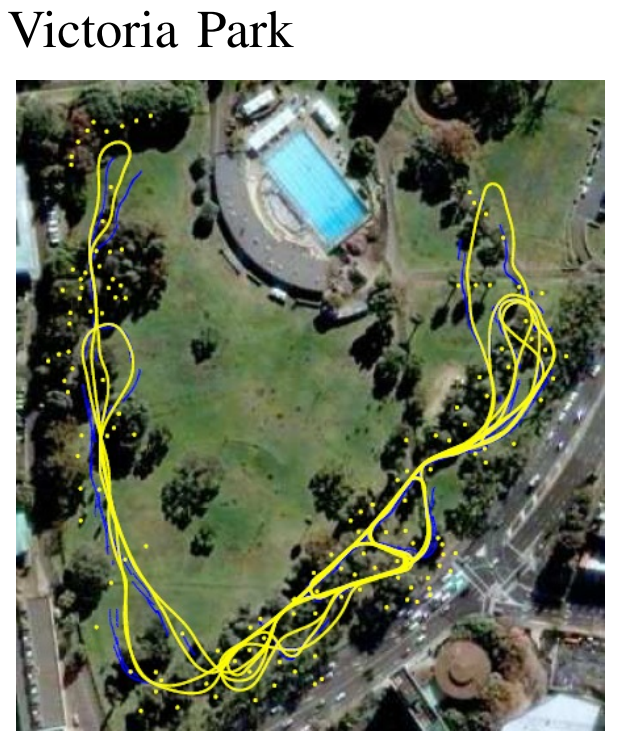
\includegraphics[width=\linewidth]{Pictures/Optimizers/iSAM2/Victoria_park_map.png}
    \caption*{\small Victoria Park \gls{SLAM} map used in the original \gls{iSAM} benchmarks.}
  \end{minipage}\hfill
  \begin{minipage}[t]{0.55\linewidth}
    \centering
    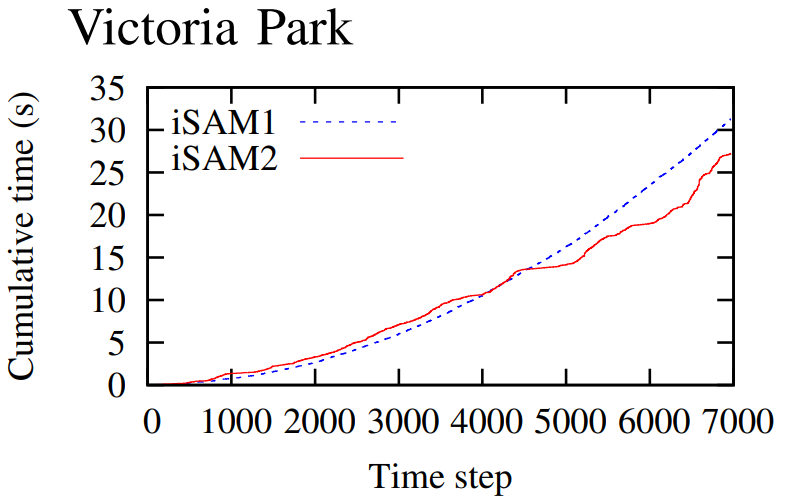
\includegraphics[width=\linewidth]{Pictures/Optimizers/iSAM2/Victoria_park_graph.png}
    \caption*{\small Cumulative time vs. step for \gls{iSAM} (periodic batch) and \gls{iSAM}2 (fluid). \gls{iSAM}2 stays faster as the dataset grows.}
  \end{minipage}
  \caption{Picture from the Bayes tree paper \cite{Bayes_tree_for_SLAM_paper}. In \gls{iSAM}2, relinearization is fluid, only the affected cliques are recomputed and the rest of the tree is reused.}
  \label{fig:optimizer-iSAM2-fluid-relin}
\end{figure}



\subsubsection{Sparse Factor Graphs}
Over long missions the factor graph can accumulate many near duplicate constraints (revisits of the same place, repeated landmark sightings from similar viewpoints). This “Eiffel Tower effect” slowly densifies the graph and enlarges cliques in the Bayes tree, which increases update cost. The fix is sparsification. Here we keep the informative constraints and summarize or drop the redundant data points while preserving the important information flow. In practice this is done locally where data arrive. We retain the freshest odometry and a few diverse loop closures, and we replace discarded constraints by a light summary on the small separator set where they would have entered the tree. Intuitively, we keep the ``shape'' of the information at the boundary and forget interior details that are now redundant. Simple policies such as keyframing (keeping only selected poses as variables), pruning highly correlated measurements, and limiting per landmark observation count work well. The result is a graph that stays sparse, cliques that stay small, and a Bayes tree that remains cheap to update even in very long runs.



\subsubsection{Beyond Gaussian Assumptions (Robust Estimators)}
Pure Gaussian residuals are fragile in the face of outliers (bad data association, spurious loop closures, moving objects, changing environment). Robust estimators fix this by replacing the quadratic loss with a robust loss that grows slower than a square. Common choices include Huber (quadratic near zero, linear in the tails), Cauchy, or Tukey. In \gls{iSAM}2 this is a drop in change at the factor level. Each robust loss yields a weight for its residual, updated as the estimate improves (iteratively re-weighted least squares). Factors that fit well keep high weight, inconsistent ones are down weighted, so they no longer dominate the solution. This makes incremental updates and fluid re-linearization safer because a single wrong constraint will not trigger large edits high up in the tree. For hard loop closures, one can also use switchable or graduated penalties that let the optimizer ``turn off'' a suspect factor until there is enough supporting evidence. The Bayes tree concept stays the same, only local factor weights and linearization adapt, so robustness comes with little extra complexity.



\subsubsection{Data Association from the Bayes Tree}
The same as in \gls{iSAM}, we score candidate matches with a Mahalanobis distance, which measures the innovation in units of its uncertainty. However in \gls{iSAM}2 the needed covariances are read directly from the Bayes tree without forming a dense matrix. Pose and nearby pose to landmark covariances are obtained efficiently by following only the few cliques that contain those variables and their separators. This keeps online/real-time gating fast for data association. Queries involving far away landmarks or many old poses may touch a larger portion of the tree and therefore cost more, but they remain practical on demand. In practice we combine a cheap, conservative bound (for routine gating) with exact small block queries when decisions are critical (eks verifying a loop closure). The result is reliable association with predictable compute cost during operation.



\subsubsection{Algorithm}
At each step we absorb new measurements, touch only the relevant cliques in the Bayes tree, solve for a small increment, and update the state. \gls{iSAM}2 combines the linear update with fluid re-linearization, so work stays local and predictable. Concretely, one iteration looks like this (matching the structure summarized in the \gls{iSAM}2 and Bayes tree papers \cite{iSAM2_paper,Bayes_tree_for_SLAM_paper})
\begin{enumerate}
    \item \textbf{Add new data:} Insert the new factors (odometry, measurements, loop closures) into the factor graph. If new states appear, add them to the estimate $\Theta$.

    \item \textbf{Mark what to refresh (fluid re-linearization):} Keep the last increment $\Delta\theta$. If a state moved more than a small threshold $\beta$, mark it for re-linearization. Only pass this mark to neighbors if the parent changed more than a smaller threshold $\alpha$. This finds the small set that really needs work now.

    \item \textbf{Build a small local problem:} Take just the cliques in the Bayes tree that touch the marked states (and their ancestors up to the root) and turn them back into a tiny factor graph, everything else becomes reusable ``orphans''.

    \item \textbf{Order and eliminate locally:} Find a sparse order for this small graph using a constrained \gls{COLAMD} (keep the newest states last, near the root), then eliminate to make a new local Bayes subtree.

    \item \textbf{Reattach orphans:} Connect the untouched subtrees back at the correct separators. Only the edited subtree changed, the rest is reused.

    \item \textbf{Solve where needed:} Back solve on the updated top of the tree to get a new increment $\Delta\theta$. Propagate the solve into children only when the parent's change is big enough (same $\alpha$ rule).

    \item \textbf{Update the estimate:} Apply the increment on the whole factor graph, $\Theta \leftarrow \Theta \oplus \Delta\Theta$ (where $\theta = \Theta$ and $\Delta\theta = \Delta\Theta$). Keep $\Delta\Theta$ for the next steps re-linearization test.

    \item \textbf{Keep variable ordering healthy (incremental):} When a loop closure grows cliques near the root, run constrained \gls{COLAMD} again, but only on that small region to reduce fill and keep the newest states near the root.
    
    \item \textbf{Data association update:} Fetch the needed local covariances from the Bayes tree, compute far away covariances only on demand, and compare predicted and observed features using our own chosen Data Association method.
\end{enumerate}



\subsubsection{Limitations}
While \gls{iSAM}2 removes the big computation spikes seen in \gls{iSAM}, some practical and theoretical limits remain.

\begin{itemize}
  \item \textbf{Ordering is heuristic, not optimal:} Choosing a variable order that minimizes fill in is NP-hard, so \gls{iSAM}2 relies on constrained \gls{COLAMD} and related heuristics. These give good, stable performance online but cannot guarantee the globally best sparsity.

  \item \textbf{Clique growth in dense areas.} Heavy revisiting of the same places (``Eiffel Tower effect'') or many near duplicate constraints can enlarge cliques near the root. Updates remain local, but the cost of each local elimination grows with clique size. In long runs we often need sparsification/keyframing to keep the graph light.

  \item \textbf{Threshold tuning for fluid re-linearization:} The accuracy/speed trade off depends on two small thresholds (who to re-linearize and how far to propagate the solve). These must be tuned for the sensor and motion model. Too loose can delay accuracy, too tight does extra work.

  \item \textbf{Faraway covariances can be expensive:} Exact marginal/covariance queries are done by recursive message passing on the tree (dynamic programming style). Queries that span long paths or large separators touch more cliques and therefore cost more.

  \item \textbf{Gaussian least-squares core:} Outliers and non Gaussian effects are not handled by \gls{iSAM}2 alone. Robust losses or switchable constraints must be added at the factor level to down weight bad data, otherwise accuracy can degrade during long missions.

  \item \textbf{Nonlinearity still matters:} Poor initial guesses or highly nonlinear measurements can require multiple Gauss-Newton/Levenberg-Marquardt steps. \gls{iSAM}2 just makes each step local.

  \item \textbf{Engineering complexity and memory:} Compared to a single global $R$ in \gls{iSAM}, the Bayes tree in \gls{iSAM}2 adds much more moving parts (cliques, separators, cached/orphan subtrees, incremental reordering). Correct, efficient implementations are more involved, and memory still grows with map size unless one prunes or summarizes.
\end{itemize}
\noindent 
In practice, most of these limits can be mitigated with careful design. Using keyframing/sparsification to cap clique size, robust losses or switchable constraints to handle outliers, and constrained incremental reordering to keep updates local. The main hurdle is engineering complexity. This is where the open source \textbf{\gls{GTSAM}} library (from the Georgia Tech team behind \gls{iSAM}/\gls{iSAM}2) is invaluable. It ships a production quality Bayes tree/\gls{iSAM}2 implementation, clean factor graph APIs, robust noise models, and utilities for ordering and re-linearization, making it a practical starting point for both research and deployment.

